\section{Tuần 2}

\subsection{Kiến trúc hệ thống}

\hspace{0.5cm} Hệ thống được thiết kế theo kiến trúc phân lớp (layered architecture), gồm bốn tầng như Hình \ref{fig:architecture}. Mỗi tầng đảm nhận một vai trò riêng biệt và giao tiếp với nhau qua các giao thức chuẩn.

\begin{figure}[H]
\centering
\begin{tikzpicture}[
    box/.style={
        rectangle, draw, rounded corners=4mm, 
        minimum width=4.2cm, minimum height=1.1cm, 
        align=center, font=\small\sffamily
    },
    labelbox/.style={
        font=\large\sffamily, align=center, inner sep=4pt
    },
    arrow/.style={->, thick, >=stealth, shorten >=3pt, shorten <=3pt},
    every node/.style={font=\large\sffamily}
]

% ==================== LAYERS ====================
% Layer 4: Giao diện
\node[box, fill=blue!15] (frontend) at (0,5.2) {Tầng giao diện\\ React + Leaflet};
\node[box, fill=blue!8] (browser) at (0,4) {Trình duyệt Web};

% Layer 3: Máy chủ
\node[box, fill=green!15] (server) at (0,2.1) {Tầng máy chủ\\ FastAPI + WebSocket};
\node[box, fill=green!8] (api) at (0,0.9) {REST API};

% Layer 2: Xử lý nhúng
\node[box, fill=yellow!15] (embedded) at (0,-1.1) {Tầng xử lý nhúng\\ Raspberry Pi};
\node[box, fill=yellow!8] (firmware) at (0,-2.8) {Firmware đọc cảm biến};

% Layer 1: Cảm biến
\node[box, fill=red!15, minimum width=2.8cm] (gps) at (-4,-5) {GPS};
\node[box, fill=red!15, minimum width=2.8cm] (imu) at (0,-5) {IMU};
\node[box, fill=red!15, minimum width=2.8cm] (laser) at (4,-5) {Laser};

% ==================== ARROWS ====================
\draw[arrow] (browser) -- node[midway, right=3pt, font=\footnotesize] {WebSocket} (server);
\draw[arrow] (api) -- node[midway, right=3pt, font=\footnotesize] {TCP/IP} (embedded);
\draw[arrow] (embedded) -- (firmware);

% Mũi tên từ Firmware xuống Sensors (phân tán rõ ràng)
\draw[arrow] (firmware) -- node[midway, left=5pt, font=\footnotesize] {UART/I2C} (gps);
\draw[arrow] (firmware) -- node[midway, right=2pt, font=\footnotesize] {I2C} (imu);
\draw[arrow] (firmware) -- node[midway, right=5pt, font=\footnotesize] {UART} (laser);

% ==================== LAYER LABELS (bên phải) ====================
\node[labelbox, text=blue!50!black] at (6.5,4.5) {Frontend\\(client)};
\node[labelbox, text=green!50!black] at (6.5,1.45) {Backend\\(server)};
\node[labelbox, text=yellow!50!black] at (6.5,-1.7) {Embedded\\(field device)};
\node[labelbox, text=red!50!black] at (6.5,-4.5) {Sensors\\(hardware)};

\end{tikzpicture}
\caption{Kiến trúc phân lớp của hệ thống}
\label{fig:architecture}
\end{figure}

\subsubsection{Tầng cảm biến (Sensor layer)}

\hspace{0.5cm} Đây là tầng thấp nhất, bao gồm phần cứng cảm biến đặt trên thiết bị di động:
\begin{itemize}
    \item \textbf{Module GPS/GNSS}: Thường là module U-Blox (NEO-6M, NEO-M8N) hoặc tương đương. Xuất dữ liệu định dạng NMEA-0183 qua UART. Tần số cập nhật 1-10 Hz. Độ chính xác 2-5 m ở chế độ dân sự.
    \item \textbf{Cảm biến IMU}: MPU6050, ICM-20948, hoặc BNO055. Tích hợp accelerometer, gyroscope, và magnetometer. Cho phép tính toán góc hướng (yaw), góc nghiêng (pitch, roll) qua giao thức I2C/SPI. Tần số cao (100-1000 Hz) nhưng cần lọc và hiệu chỉnh nhiệt.
    \item \textbf{Laser rangefinder}: LIDAR-Lite v3 (40 m, phù hợp ngoài trời), TF-Luna (8 m), hoặc VL53L1X (ToF, tầm 4 m, phù hợp trong nhà). Với yêu cầu theo dõi đến 1000 m ngoài trời, LIDAR-Lite v3 là lựa chọn phù hợp hơn. Đo khoảng cách bằng phương pháp Time-of-Flight. Độ chính xác +/- 1-2 cm, nhưng phụ thuộc vào màu sắc và kết cấu bề mặt mục tiêu.
\end{itemize}

\subsubsection{Tầng xử lý nhúng (Embedded layer)}

\hspace{0.5cm} Raspberry Pi (RPi 3B+ hoặc 4B) đóng vai trò là bộ điều khiển trung tâm (central hub) kết nối các cảm biến. RPi chạy hệ điều hành Raspberry Pi OS (Linux-based). Phần mềm đọc cảm biến được viết bằng Python.

Vai trò chính của RPi:
\begin{itemize}
    \item Đọc dữ liệu từ GPS qua UART (giao tiếp serial).
    \item Đọc dữ liệu từ IMU qua I2C.
    \item Đọc dữ liệu từ laser rangefinder qua I2C.
    \item Đóng gói dữ liệu thành định dạng JSON.
    \item Gửi dữ liệu lên máy chủ qua kênh truyền dữ liệu hai chiều (Wi-Fi hoặc Ethernet).
    \item (Tương lai) Thực hiện xử lý sơ bộ như lọc nhiễu, kiểm tra lỗi.
\end{itemize}

\subsubsection{Tầng máy chủ (Server layer)}

\hspace{0.5cm} Máy chủ được xây dựng bằng FastAPI, một framework Python hiện đại hỗ trợ bất đồng bộ (async). Các chức năng:
\begin{itemize}
    \item \textbf{REST API}: Cho phép khởi tạo phiên (session), dừng phiên, truy vấn lịch sử dữ liệu. Định dạng trả về là JSON.
    \item \textbf{WebSocket}: Kênh giao tiếp hai chiều thời gian thực. Raspberry Pi gửi dữ liệu cảm biến lên, server xử lý và gửi kết quả xuống giao diện.
    \item \textbf{Bộ tính toán}: Thực hiện phép chuyển đổi tọa độ (WGS84, ECEF, ENU, Body frame), tính toán vị trí mục tiêu.
    \item \textbf{Bộ lọc}: Kalman filter và Alpha-beta filter để ước lượng trạng thái.
    \item \textbf{Quản lý phiên}: Lưu trạng thái phiên (đang hoạt động, đã dừng), thông số cấu hình, lịch sử tọa độ.
\end{itemize}

\subsubsection{Tầng giao diện (Frontend layer)}

\hspace{0.5cm} Giao diện người dùng chạy trên trình duyệt web, sử dụng React và Vite để đóng gói. Các thành phần chính:
\begin{itemize}
    \item \textbf{Bản đồ}: Thư viện Leaflet hiển thị bản đồ OpenStreetMap. Vị trí người quan sát được đánh dấu xanh, vị trí mục tiêu đánh dấu đỏ. Leaflet đáp ứng tốt cho bản đồ 2D; bản đồ 3D với CesiumJS có thể được bổ sung nếu yêu cầu đề tài mở rộng.
    \item \textbf{Lớp thông tin}: Hiển thị tọa độ, góc ngắm, khoảng cách, tốc độ, trạng thái hệ thống.
    \item \textbf{Biểu đồ}: Hiển thị độ cao, sai số, quỹ đạo theo thời gian.
    \item \textbf{Điều khiển phiên}: Các nút bật/tắt bám mục tiêu, cấu hình tham số.
\end{itemize}

\subsection{Nguyên lý hoạt động}

\hspace{0.5cm} Hoạt động của hệ thống được mô tả bằng các bước sau:

\subsubsection{Luồng dữ liệu tổng quát}

\begin{enumerate}
    \item Raspberry Pi đọc dữ liệu từ ba cảm biến (GPS, IMU, Laser) theo chu kỳ đều đặn (ví dụ mỗi 50 ms).
    \item Dữ liệu thô được chuẩn hóa: GPS chuyển sang tọa độ thập phân, IMU tính góc hướng, laser lấy giá trị khoảng cách.
    \item RPi đóng gói bộ ba dữ liệu này thành một bản tin JSON:
\begin{verbatim}
{
  "timestamp": 1718400000.123,
  "gps": {"lat": 10.7625, "lon": 106.6602, "alt": 15.0},
  "imu": {"azimuth": 45.0, "elevation": 10.0},
  "laser": {"distance": 125.0}
}
\end{verbatim}
    \item Bản tin JSON được gửi lên máy chủ qua kênh truyền dữ liệu hai chiều.
    \item Máy chủ nhận dữ liệu, thực hiện:
    \begin{itemize}
        \item Chuyển đổi GPS từ WGS84 sang ECEF, rồi sang ENU.
        \item Tạo vector định hướng 3D từ azimuth và elevation.
        \item Nhân vector định hướng với khoảng cách laser để được tọa độ tương đối.
        \item Cộng vào vị trí người quan sát để được tọa độ mục tiêu trong ENU.
        \item Chuyển đổi ngược về WGS84.
        \item Áp dụng Kalman filter hoặc alpha-beta để ước lượng.
    \end{itemize}
    \item Tọa độ mục tiêu đã xử lý được gửi xuống giao diện qua kênh truyền dữ liệu hai chiều.
    \item Giao diện cập nhật vị trí mục tiêu trên bản đồ.
\end{enumerate}

\subsubsection{Chuyển đổi tọa độ}

\hspace{0.5cm} Một trong những thành phần quan trọng nhất của hệ thống là chuyển đổi tọa độ. Đầu vào là tọa độ WGS84 của người quan sát. Đầu ra cũng là WGS84 nhưng của mục tiêu. Ở giữa, cần chuyển qua nhiều hệ trung gian:

\begin{equation}
\begin{aligned}
\text{WGS84} &\xrightarrow{(1)} \text{ECEF} \\
\text{ECEF} &\xrightarrow{(2)} \text{ENU (tại vị trí người quan sát)} \\
\text{ENU} &\xrightarrow{(3)} \text{Cộng vector định hướng $\cdot$ khoảng cách} \\
\text{Kết quả} &\xrightarrow{(4)} \text{WGS84}
\end{aligned}
\end{equation}

Bước (1) và (4) sử dụng công thức chuyển đổi giữa WGS84 và ECEF đã được trình bày trong Phase 1. Bước (2) sử dụng ma trận xoay được xây dựng từ kinh độ và vĩ độ. Bước (3) là phép tính vector:

\begin{equation}
\mathbf{p}_{target} = \mathbf{p}_{observer} + d \cdot \mathbf{v}(\alpha, \beta)
\end{equation}

Trong đó $d$ là khoảng cách laser, $\alpha$ là azimuth, $\beta$ là elevation, $\mathbf{v}$ là vector đơn vị hướng.

Sơ đồ lớp (class diagram) mô tả các thực thể phần mềm chính và mối quan hệ giữa chúng được trình bày trong Hình \ref{fig:class}.

\newpage

\begin{figure}[htbp]
\centering
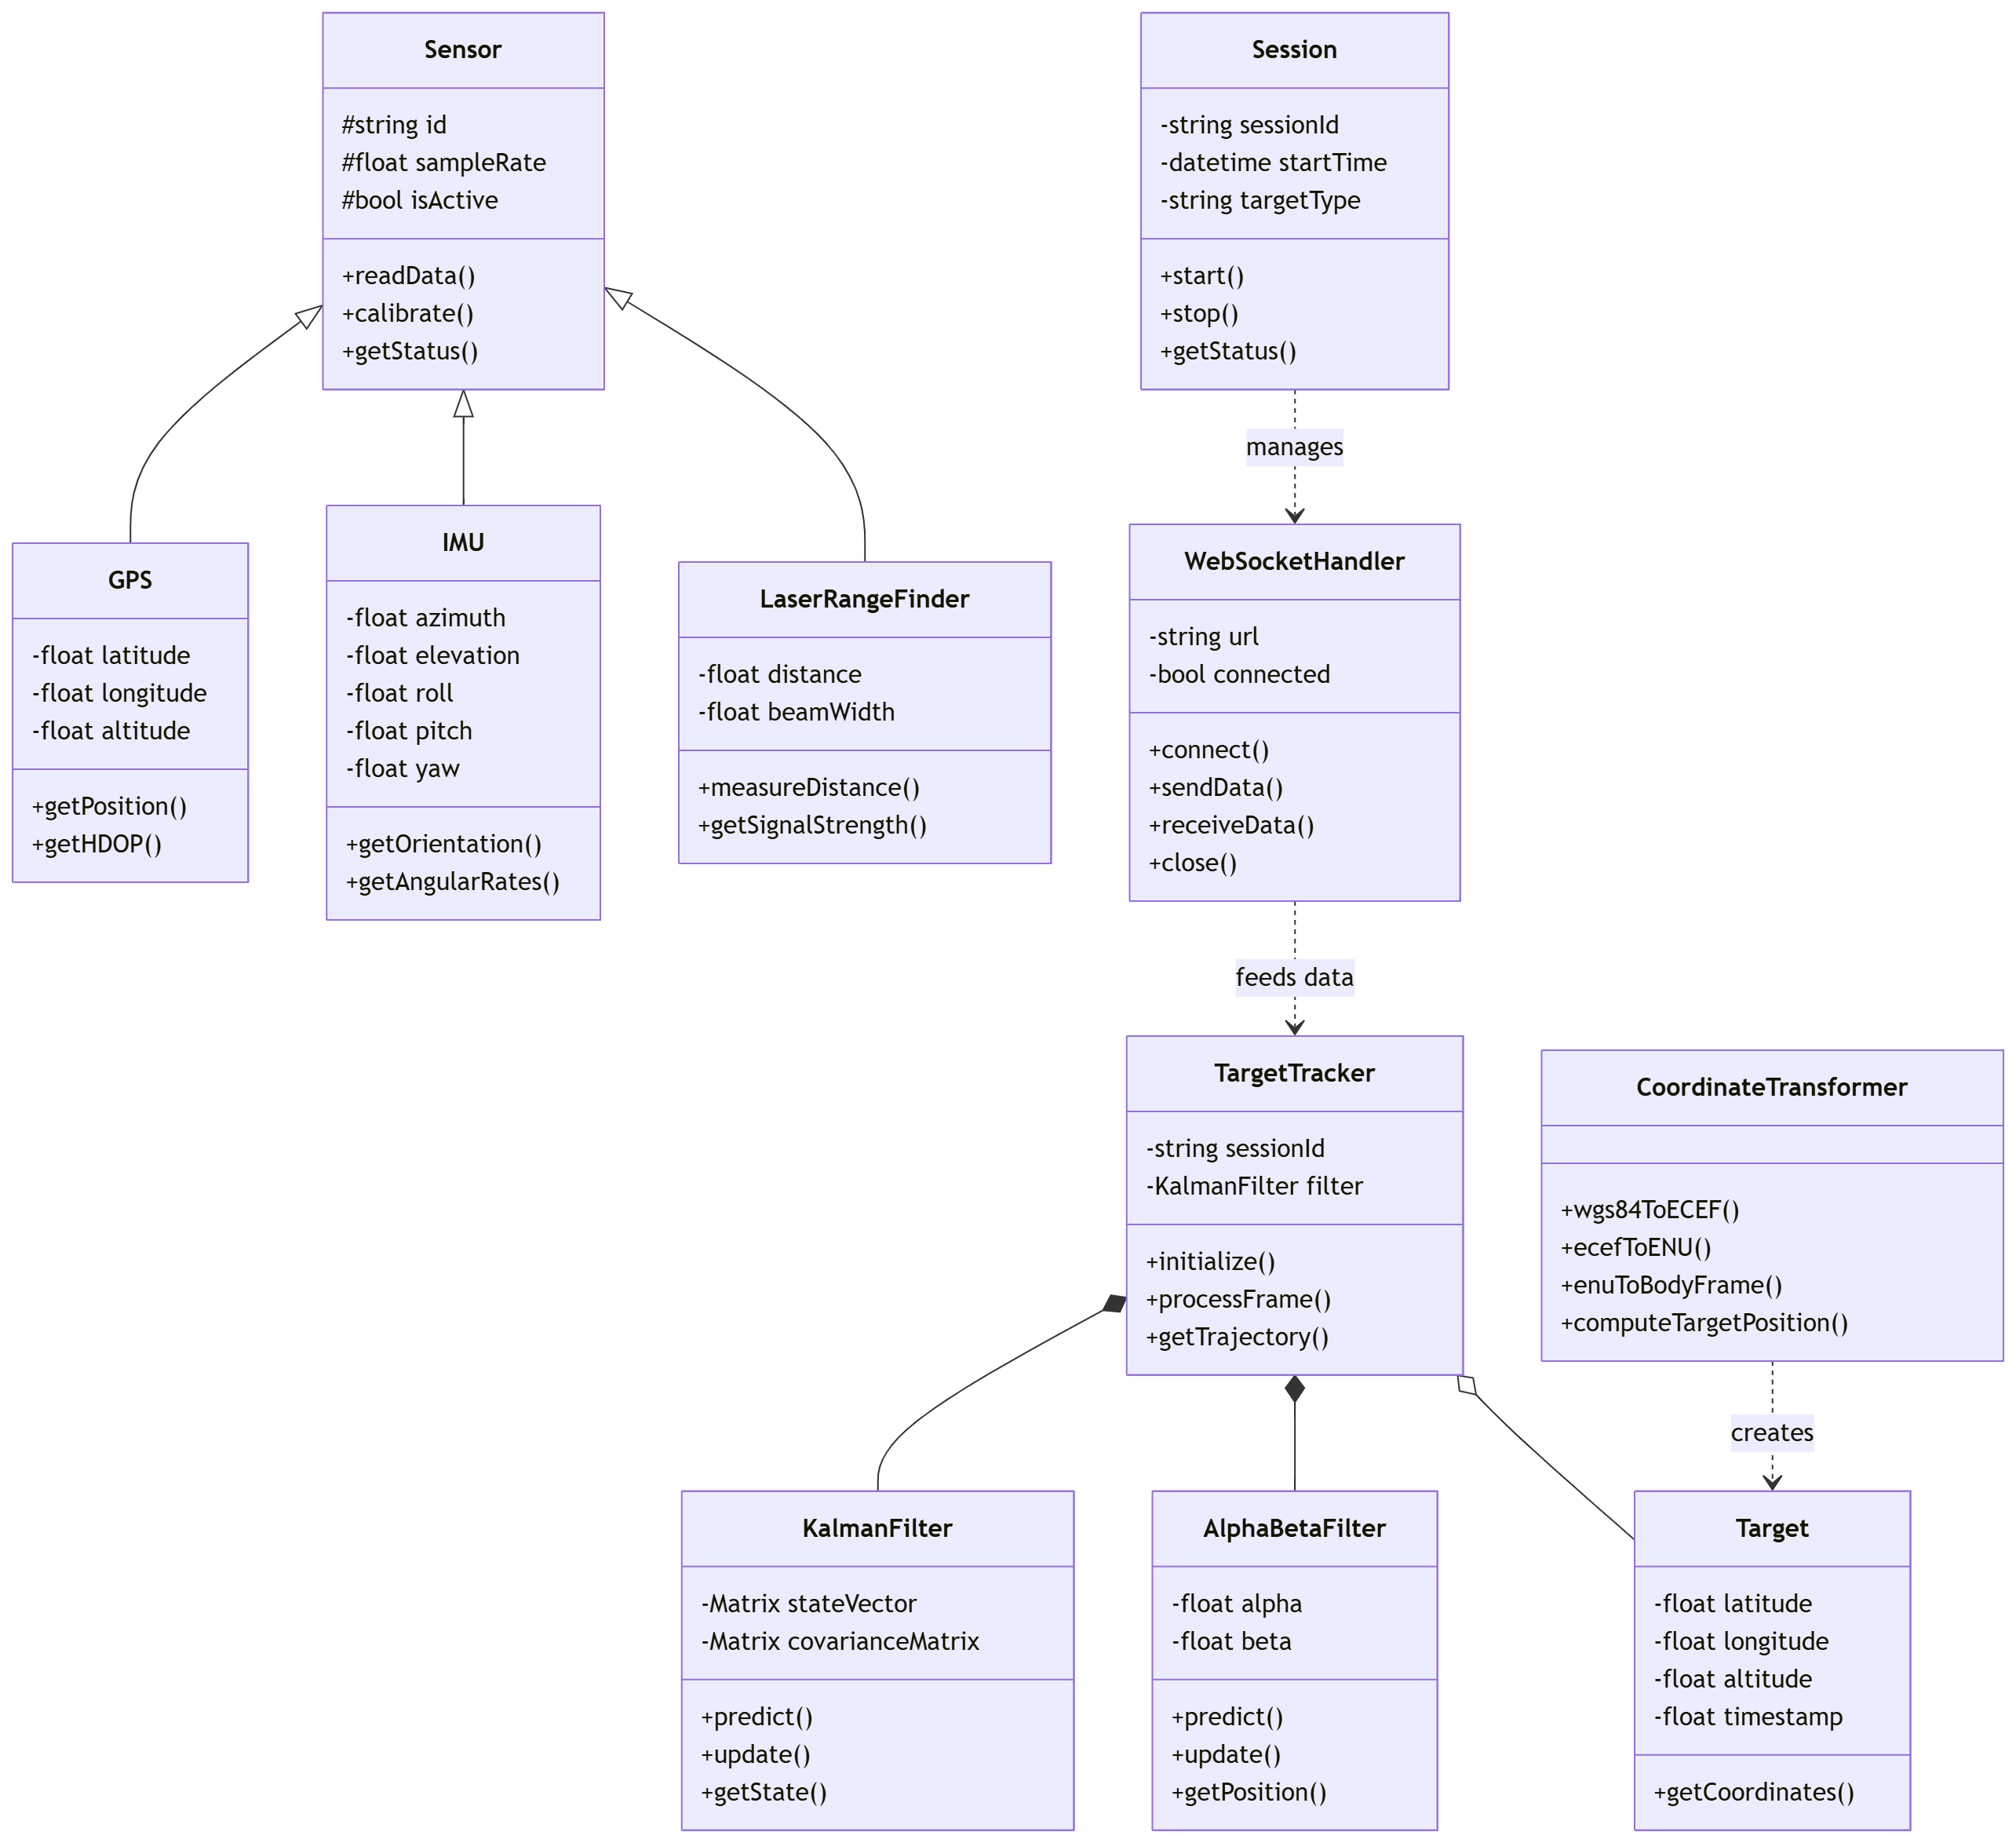
\includegraphics[width=0.9\textwidth]{Images/class-diagram.png}
\caption{Sơ đồ lớp của hệ thống phần mềm}
\label{fig:class}
\end{figure}

\subsection{Sơ đồ hoạt động (Activity diagram)}

\hspace{0.5cm} Hệ thống có hai quy trình hoạt động chính được mô tả bằng các activity diagrams.

\subsubsection{Quy trình xử lý dữ liệu}

\hspace{0.5cm} Hình \ref{fig:activity-processing} mô tả quy trình xử lý dữ liệu từ lúc đọc cảm biến đến khi xuất tọa độ. Dữ liệu từ GPS, IMU, và laser được đọc đồng thời. Sau đó kiểm tra tính hợp lệ. Nếu hợp lệ, thực hiện chuyển đổi tọa độ, tính vector định hướng, nhân với khoảng cách, áp dụng bộ lọc, và xuất kết quả. Nếu không hợp lệ, ghi nhận lỗi và gửi cảnh báo.

\newpage

\begin{figure}[htb!]
\centering
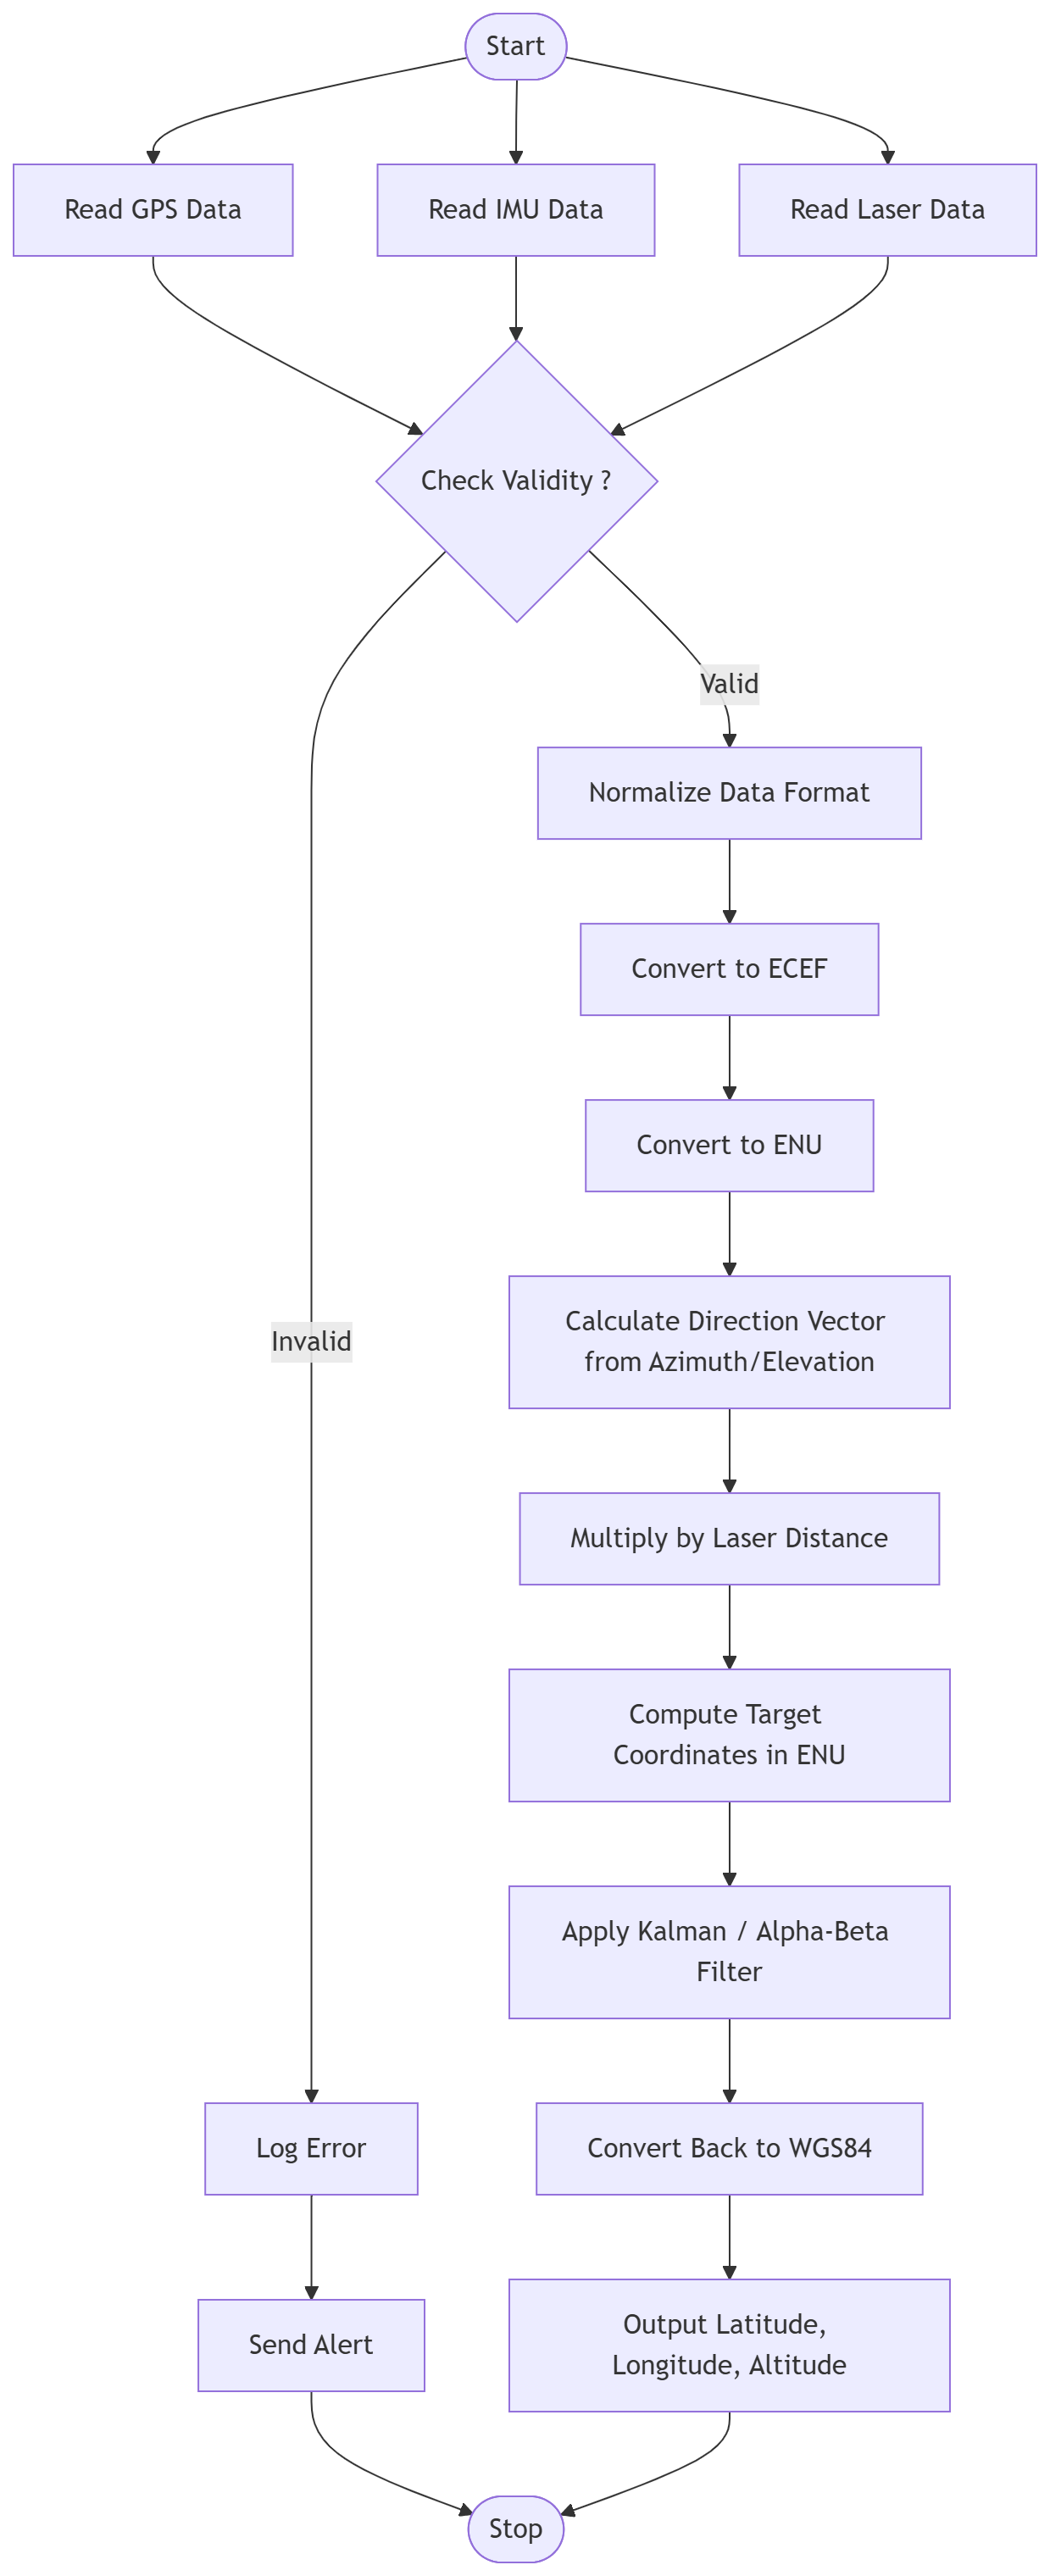
\includegraphics[width=0.55\textwidth]{Images/activity-diagram.png}
\caption{Quy trình xử lý dữ liệu từ cảm biến đến tọa độ mục tiêu}
\label{fig:activity-processing}
\end{figure}

\subsubsection{Quy trình tracking}

\hspace{0.5cm} Hình \ref{fig:activity-tracking} mô tả quy trình tracking từ lúc bắt đầu phiên đến khi kết thúc. Người dùng khởi tạo phiên, hệ thống kết nối kênh truyền dữ liệu hai chiều. Sau đó vào vòng lặp tracking: đọc cảm biến, tính toán, cập nhật bản đồ. Nếu mất tín hiệu, hệ thống chuyển sang chế độ ước lượng từ bộ lọc. Nếu người dùng yêu cầu dừng, vòng lặp kết thúc, lộ trình được lưu lại.

\begin{figure}[htb!]
\centering
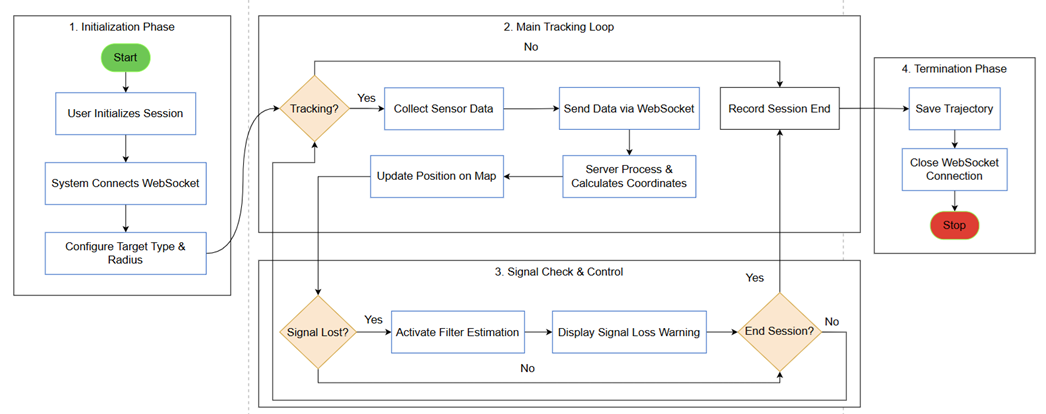
\includegraphics[width=1\textwidth]{Images/activity-tracking.png}
\caption{Quy trình tracking thời gian thực}
\label{fig:activity-tracking}
\end{figure}

\subsection{Xử lý nhúng với Raspberry Pi}

\hspace{0.5cm} Raspberry Pi được chọn làm nền tảng xử lý nhúng vì những lý do sau:
\begin{itemize}
    \item Phù hợp cho những dự án phức tạp, cần xử lý đa tác vụ.
    \item Hệ điều hành Linux đầy đủ, hỗ trợ nhiều ngôn ngữ lập trình.
    \item Nhiều chân GPIO: UART, I2C, SPI để kết nối cảm biến.
    \item Khi dự án cần kết nối Internet phức tạp và giao diện đồ họa đẹp mắt.
    \item Cộng đồng lớn, tài liệu phong phú.
\end{itemize}

Thiết kế dự kiến:
\begin{itemize}
    \item GPS module kết nối qua chân UART (pin GPIO 14/15). Đọc dữ liệu NMEA bằng thư viện giao tiếp serial.
    \item IMU kết nối qua I2C (pin GPIO 2/3). Đọc dữ liệu bằng thư viện I2C.
    \item Laser rangefinder kết nối qua UART hoặc I2C.
    \item Ứng dụng Python chạy độc lập, đọc cảm biến theo chu kỳ, gửi dữ liệu qua kênh truyền dữ liệu hai chiều.
\end{itemize}

Phần xử lý nhúng này được thiết kế để hoạt động độc lập, không cần máy tính. Người dùng mang Raspberry Pi gắn trên bảng điều khiển, tripod hoặc túi đeo ra hiện trường, bật nguồn là hệ thống tự động chạy. Dữ liệu được gửi về máy chủ trung tâm qua mạng Wi-Fi hoặc 4G nếu có USB dongle.

Kết quả được kiểm chứng qua mô phỏng với mô hình nhiễu Gaussian, sử dụng công cụ mô phỏng quỹ đạo tích hợp trong hệ thống. Phương pháp này cho phép kiểm soát điều kiện thử nghiệm và lặp lại kết quả, phù hợp cho giai đoạn đánh giá thuật toán. Vị trí GPS được sinh theo quỹ đạo định trước, góc ngắm và khoảng cách được mô phỏng dựa trên vị trí thực của mục tiêu kết hợp với mô hình nhiễu cảm biến.
